\documentclass[12pt,letterpaper]{article}
\usepackage{graphicx,textcomp}
\usepackage{natbib}
\usepackage{setspace}
\usepackage{fullpage}
\usepackage{color}
\usepackage[reqno]{amsmath}
\usepackage{amsthm}
\usepackage{fancyvrb}
\usepackage{amssymb,enumerate}
\usepackage[all]{xy}
\usepackage{endnotes}
\usepackage{lscape}
\newtheorem{com}{Comment}
\usepackage{float}
\usepackage{hyperref}
\newtheorem{lem} {Lemma}
\newtheorem{prop}{Proposition}
\newtheorem{thm}{Theorem}
\newtheorem{defn}{Definition}
\newtheorem{cor}{Corollary}
\newtheorem{obs}{Observation}
\usepackage[compact]{titlesec}
\usepackage{dcolumn}
\usepackage{tikz}
\usetikzlibrary{arrows}
\usepackage{multirow}
\usepackage{xcolor}
\newcolumntype{.}{D{.}{.}{-1}}
\newcolumntype{d}[1]{D{.}{.}{#1}}
\definecolor{light-gray}{gray}{0.65}
\usepackage{url}
\usepackage{listings}
\usepackage{color}

\definecolor{codegreen}{rgb}{0,0.6,0}
\definecolor{codegray}{rgb}{0.5,0.5,0.5}
\definecolor{codepurple}{rgb}{0.58,0,0.82}
\definecolor{backcolour}{rgb}{0.95,0.95,0.92}

\lstdefinestyle{mystyle}{
	backgroundcolor=\color{backcolour},   
	commentstyle=\color{codegreen},
	keywordstyle=\color{magenta},
	numberstyle=\tiny\color{codegray},
	stringstyle=\color{codepurple},
	basicstyle=\footnotesize,
	breakatwhitespace=false,         
	breaklines=true,                 
	captionpos=b,                    
	keepspaces=true,                 
	numbers=left,                    
	numbersep=5pt,                  
	showspaces=false,                
	showstringspaces=false,
	showtabs=false,                  
	tabsize=2
}
\lstset{style=mystyle}
\newcommand{\Sref}[1]{Section~\ref{#1}}
\newtheorem{hyp}{Hypothesis}
\UseRawInputEncoding

\title{Problem Set 7: QTM 200 Applied Regression Analysis}
\date{Due: May 6, 2020}
\author{Farris Sabir}

\begin{document}
	\maketitle
	
	\section*{Instructions}
	\begin{itemize}
		\item Please show your work! You may lose points by simply writing in the answer. If the problem requires you to execute commands in \texttt{R}, please include the code you used to get your answers. Please also include the \texttt{.R} file that contains your code. If you are not sure if work needs to be shown for a particular problem, please ask.
		\item Your homework should be submitted electronically on the course GitHub page in \texttt{.pdf} form.
		\item This problem set is due before midnight on Wednesday, May 6, 2020. No late assignments will be accepted.
		\item Total available points for this homework is 100.
	\end{itemize}
	
	\vspace{.5cm}

\section*{Question 1 (50 points): Political Science}	
\noindent Consider the data set \texttt{MexicoMuniData.csv}, which includes municipal-level information from Mexico. The outcome of interest is the number of times the winning PAN presidential candidate in 2006 (\texttt{PAN.visits.06}) visited a district leading up to the 2009 federal elections, which is a count. Our main predictor of interest is whether the district was highly contested, or whether it was not (the PAN or their opponents have electoral security) in the previous federal elections during 2000 (\texttt{competitive.district}), which is binary (1=close/swing district, 0="safe seat"). We also include \texttt{marginality.06} (a measure of poverty) and \texttt{PAN.governor.06} (a dummy for whether the state has a PAN-affiliated governor) as additional control variables. 

\lstinputlisting[language=R, firstline=46, lastline=46]{PS07.R}  

\begin{enumerate}
	\item [(a)]
	Run a Poisson regression because the outcome is a count variable. Is there evidence that PAN presidential candidates visit swing districts more? Provide a test statistic and p-value.
	
	\lstinputlisting[language=R, firstline=49, lastline=66]{PS07.R}  
	
	There is no statistically reliable evidence that PAN presidential candidates visit swing districts more or less. The z-statistic from the Poisson regression's estimate of -0.4594 is -1.402, which has an associated p-value of 0.161. This is not statistically significant and would lead to failing to reject the null hypothesis that PAN presidential candidates visit swing districts more.
	
	\item [(b)]
	Interpret the \texttt{marginality.06} and \texttt{PAN.governor.06} coefficients.
	
	\lstinputlisting[language=R, firstline=72, lastline=76]{PS07.R}  
	
	The marginality.06 coefficient of -2.0981 means that the average number of times the winning PAN presidential candidate in 2006 visited a district before 2009 federal elections decreases as poverty increases. Specifically, as poverty increases by a unit of one on this scale, holding all else equal, the average number of visits decreases by a multiplicative factor of 0.1226841. Also, the PAN.governor.06 coefficient of -0.2073 means that the average number of times the winning PAN presidential candidate in 2006 visited a district before 2009 federal elections decreases when switching from a state with a PAN-affiliated governor to a state without one. Specifically, holding all else equal, switching from a state without a PAN\_affiliated governor to a state with one means the average number of visits decreases by a multiplicative factor of 0.8127638.
	
	
	\item [(c)]
	Provide the estimated mean number of visits from the winning PAN presidential candidate for a hypothetical district that was competitive (\texttt{competitive.district}=1), had an average poverty level (\texttt{marginality.06} = 0), and a PAN governor (\texttt{PAN.governor.06}=1).
	
	\lstinputlisting[language=R, firstline=83, lastline=84]{PS07.R}  
	
	Therefore, the estimated mean number of visits is 0.01, which rounds to zero or no visits on average.
	
	
\end{enumerate}
	

\section*{Question 2 (50 points): Biology}
\noindent We'll be using data from a longitudinal sleep study of under 20 undergraduate students ($n$=18), which took place over the course of 10 days to see if sleep deprivation has any effect on participants' reaction time. Load the data through the \texttt{lmer} package.

\lstinputlisting[language=R, firstline=91, lastline=91]{PS07.R}  

\begin{enumerate}
	\item
	Create a "pooled" linear model where you regress \texttt{Days} on the outcome \texttt{Reaction}. Make sure to run regression diagnostics to check if the variance around the regression line is equal for every year.
	
	\lstinputlisting[language=R, firstline=93, lastline=108]{PS07.R}  
	
	\begin{figure}[h!]
		\caption{\footnotesize{Diagnostic Plots}}
		\vspace{.5cm}
		\centering
		\label{fig:diagnosticplots}
		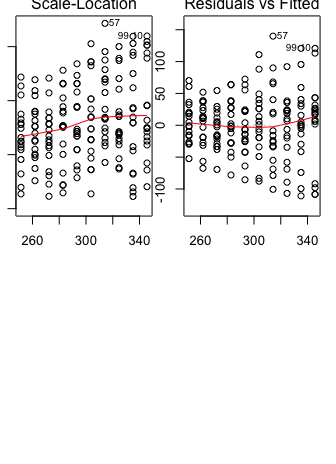
\includegraphics[width=1\textwidth]{./PS7_Plot_1.png}
	\end{figure}	
	
	The diagnostic plots are shown in Figure 1. The scale location plot helps us verify that the variance is relatively constant with a straight horizontal line. The residuals vs. fitted values plot also helps us see equal spread across most fitted values.
	
	\item Fit an "un-pooled" regression model with varying intercepts for patient (include an additive factor for patient) and save the fitted values.
	
	\lstinputlisting[language=R, firstline=113, lastline=143]{PS07.R}  
	
	\item Fit a "un-pooled" regression model with varying slopes of time (days) for patients (include only the interaction \texttt{Days:Subject}) and save the fitted values.
	
	\lstinputlisting[language=R, firstline=146, lastline=175]{PS07.R}  
	
	\item Fit an "un-pooled" regression model with varying intercepts for patients with varying slopes of time (days) by patient (include the interaction and constituent terms of \texttt{Days} and \texttt{Subject}, \texttt{Days + Subject + Days:Subject}) and save the fitted values.
	
	\lstinputlisting[language=R, firstline=178, lastline=225]{PS07.R}  
	
	\item Fit a "semi-pooled" multi-level model with varying-intercept for subject and varying-slope of day by subject. Is it worthwhile for us to run a multi-level model with varying effects of time by subject? Why? Compare your model from part 5 to the other completely "pooled" or "un-pooled models".
	
	\lstinputlisting[language=R, firstline=228, lastline=252]{PS07.R}  
	
	\begin{figure}[h!]
		\caption{\footnotesize{Comparing Models}}
		\vspace{.5cm}
		\centering
		\label{fig:diagnosticplots}
		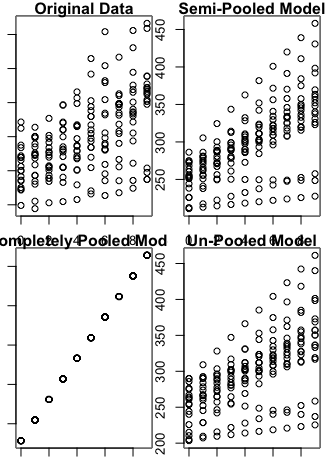
\includegraphics[width=1\textwidth]{./PS7_Plot_2.png}
	\end{figure}
	
	According to Figure 2, the multi-level model seems really similar to the un-pooled model except that pooling is invovled. The multi-level model truly falls in between the completely and unpooled model in that it has pooling, but the chances are not equal in between days, like it is for the completely pooled model. This may provide the benefit of being able to manipulate levels in a structured way compared to unpooled model, but also providing some information as each unit has a different chance of success.
	
	

\end{enumerate}

\end{document}
